\documentclass[11pt]{article}

\usepackage[a4paper,margin=1in]{geometry}
\usepackage{amsmath,amssymb,siunitx}
\usepackage{enumitem,booktabs,hyperref,tcolorbox,xspace,graphicx}
\setlist{nosep}

\newcommand{\code}[1]{\texttt{#1}}
\newcommand{\term}[1]{\textbf{#1}}

\begin{document}

\begin{center}
  {\LARGE \textbf{Project Option -- GPU Wavelets (JPEG2000-style MRA)}}\\[0.25em]
  \small GPU Computing (Master), bonus project
\end{center}

\vspace{0.6em}

\begin{tcolorbox}[colback=gray!6,colframe=gray!50!black]
\textbf{Goal.} Starting from the provided 1D CPU reference (\code{1D\_wavelets.cpp}), implement a fully GPU-accelerated wavelet transform and a simple multi-resolution representation (MRA) in the style of JPEG2000. Develop from a minimal 1D baseline (analysis + synthesis) into an efficient 2D GPU implementation.
\end{tcolorbox}

\section*{General Project Guidelines}

\begin{tcolorbox}[colback=gray!6,colframe=gray!50!black]
The following guidelines apply to all projects.
\end{tcolorbox}

\subsection*{Scope \& Spirit}
Projects are meant to deepen your understanding of GPU computing through a concrete, measurable task.
You may \textbf{deviate} from the suggested items if you have a better idea, provided it stays within the \emph{spirit} of the project (same learning goals).
If you wish to propose a new scoring item not listed, \textbf{ask for approval} first; I will grant it if it has clear pedagogical value.

\subsection*{Deliverables}
\begin{enumerate}[label=\arabic*.]
    \item \textbf{Repository (required).} CUDA/C++ code with a clear structure and clear build/run instructions (e.g., in a \code{README.md}). Ideally, an automated build system (e.g., \code{CMakeLists.txt}).
    \item \textbf{Report (required).} Either \emph{Markdown} (in the repo) or a \emph{PDF} (3--10 pages). It should focus on:
    \begin{itemize}
        \item What you implemented (which items, with brief descriptions).
        \item Performance discussion: methodology, measurements, what limits throughput.
        \item Design/implementation choices: data layout, synchronization methods, trade-offs.
        \item Anything worth a discussion (e.g., failed attempts, unexpected findings).
    \end{itemize}
\end{enumerate}
Please note that the report is as important as the code for the assessment.

\subsection*{Submission \& Deadlines}
\begin{tcolorbox}[colback=white,colframe=black!10,title=Deadlines]
\textbf{Mid-semester feedback (optional):} \emph{July 17, 2026} (Sun), 23:59 CET.\\
\textbf{Hard deadline:} \emph{July 31, 2026} (Sun), 23:59 CET.
\end{tcolorbox}

\paragraph{Mid-semester feedback (optional).}
Submit a draft by July 17 to get written feedback from me:
\begin{itemize}
    \item Are you on track to reach the threshold (bonus) if submitted as is?
    \item Are you heading in a sensible technical direction?
    \item Any major flaw or mismatch with course goals?
    \item If your chosen direction is off-topic for the course, I will say so here.
\end{itemize}

\subsection*{Submission Workflow}
\begin{enumerate}[label=\arabic*.]
    \item Host the code on the LRZ GitLab. \textbf{Fork} the course repo (or create your own), open a \textbf{Merge Request}, and \textbf{assign me as reviewer}. If anything special should be noted you can add a short description in the MR.
    \item If you do not have LRZ GitLab access, email me a link to your repository.
\end{enumerate}

\subsection*{Evaluation}
\begin{itemize}
    \item \textbf{Grading.} Evaluation is \emph{pass/fail} based on the sum of points from the project's item list.
        Each item has a stated value; you can earn \emph{full}, \emph{partial}, or \emph{no} credit depending on the quality of your implementation and evidence.
        If your total is \textbf{$\geq$ 50 points}, you \textbf{pass} and receive a \textbf{--0.3} bonus on the final grade; otherwise, no bonus is awarded.
        The projects' maximum amount of points \textbf{exceeds} 50 and you do \textbf{not} need to implement everything and should rather pick the items that best fit your interests and time.
        Please mention in the report which items you implemented.
        Items completed with more depth or quality may receive \emph{extra} points at my discretion.
    \item \textbf{Workload expectation.} The bonus is calibrated for \(\approx\)20 hours of effective work \emph{per student}. Your submission should reflect this depth (code, measurements, and report).
    \item \textbf{What I value.} Code correctness first, then correct reasoning, then performance.
        Please note that it is still interesting if an optimization attempt \emph{fails} to deliver speedup, moreso if you can explain \emph{why}.
    \item \textbf{Evidence.} Include timing tables, plots, or other measurements for all relevant items.
        Detail as much as possible your measurement methodology (e.g., warmup, averaging, input sizes).
        Performance-related items will not be awarded points without evidence.
\end{itemize}

\subsection*{General Rules}
\begin{itemize}
    \item Your work will be assessed individually. You may collaborate with classmates for discussion, but the code and report must be your own.
    \item The use of AI tools is permitted but you will be held accountable for your submission.
    \item Unless specified otherwise, you are expected to propose pure CUDA kernels without using external libraries (e.g., Thrust, cuBLAS).
            Occasional, well-justified library calls are acceptable; in particular, in-kernel CUB collectives (e.g., \code{cub::WarpScan}, \code{cub::BlockScan}, \code{cub::BlockReduce}) are permitted.
            Avoid relying on host-side opaque primitives (e.g., \code{thrust::exclusive\_scan}, \code{cub::DeviceScan}) for your solution, although it is recommended to compare against them when appropriate (and it is perfectly fine to be slower).
            The objective of this project is to demonstrate kernel-level design (memory hierarchy, synchronization, divergence).
\end{itemize}

\begin{tcolorbox}[colback=gray!6,colframe=gray!50!black,title=Quick Checklist]
\begin{itemize}
    \item The \emph{readme} or \emph{report} explains how to compile and run your code.
    \item Following the instructions indeed builds and runs the code.
    \item There is a report (Markdown or PDF) covering implementation, measurements, and analysis.
    \item Submission via GitLab MR (assigned to me) or, if unavailable, by email with a link.
\end{itemize}
\end{tcolorbox}


\section*{Introduction}

Wavelet transforms are a broad family of techniques that decompose signals into different scale components.
Separable wavelet transforms are widely used in image processing and compression (e.g., JPEG2000) because they include useful properties that we will not detail here.
One such property is the ability to perform multi-resolution analysis (MRA), which decomposes an image into a hierarchy of frequency subbands at multiple scales.

\begin{figure}[h]
  \centering
  \begin{tabular}{cc}
    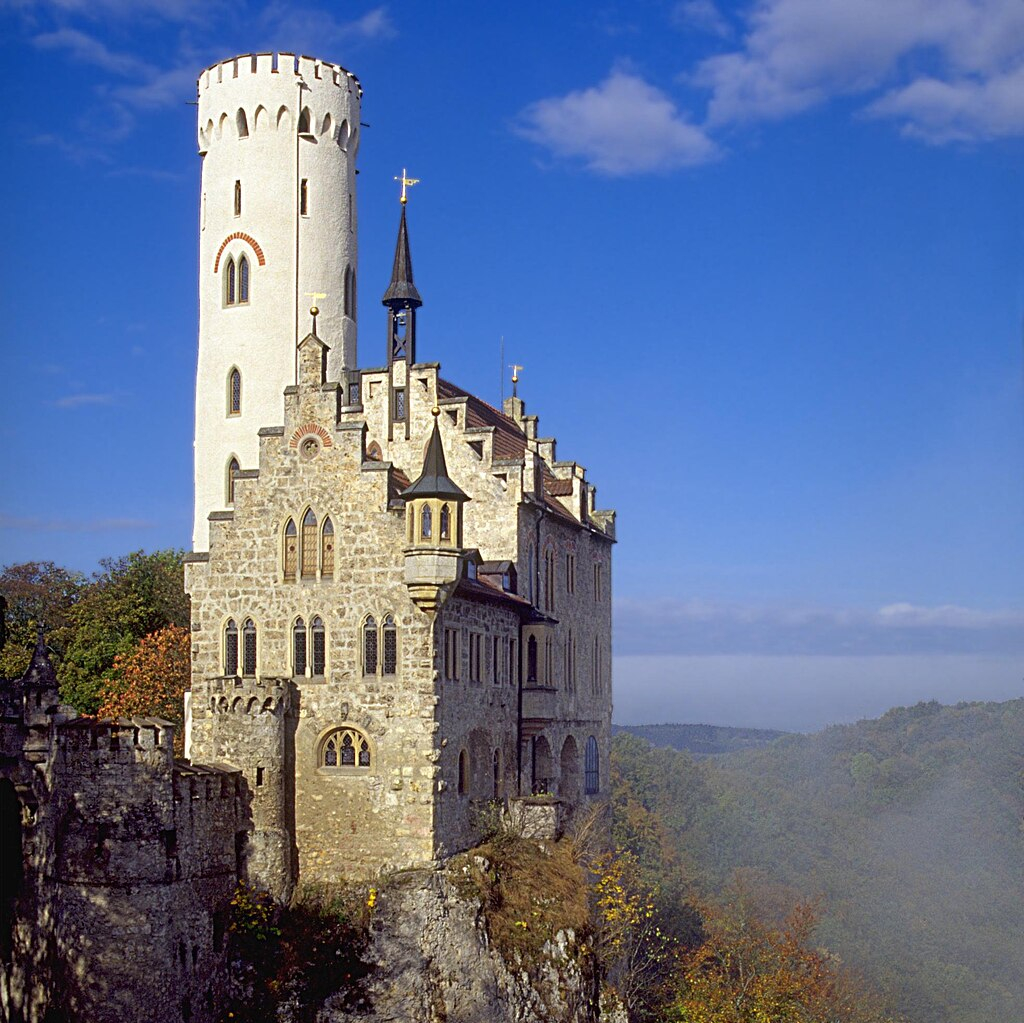
\includegraphics[width=0.4\textwidth]{assets/Castle_Lichtenstein.jpg} &
    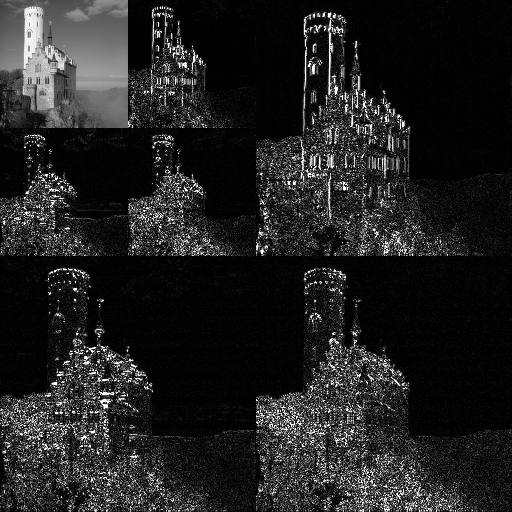
\includegraphics[width=0.4\textwidth]{assets/Castle_Lichtenstein_MRA.png} \\
    (a) Original image & (b) Multi-resolution representation (MRA)
  \end{tabular}
  \caption{(a) Original image and (b) its multi-resolution representation via wavelets.
  By applying the same transform recursively (MRA), we obtain a hierarchical decomposition
  of the image into different frequency subbands at multiple scales.}
  \label{fig:mra_example}
\end{figure}

In Figure~\ref{fig:mra_example}, we see an example of an image and its MRA representation obtained via separable wavelets.
To obtain this image, we can apply the following steps:
\begin{enumerate}[leftmargin=1.5em]
  \item \term{1D transform.} Implement the forward and inverse wavelet scheme in one dimension (1D). This 1D transform is provided in the baseline code \code{1D\_wavelets.cpp}.
  \item \term{2D separable transform.} By applying the 1D transform first along all the rows and then along the columns of an image, we obtain a 2D image with 4 quadrants (subbands): \textsf{LL} (low-low), \textsf{HL} (high-low), \textsf{LH} (low-high), and \textsf{HH} (high-high).
        The \textsf{LL} subband contains a coarse approximation of the image, while the other three subbands capture different orientations of detail.
        \textit{Note:} The order can also be columns first, then rows; the result is the same.
  \item \term{Multi-level MRA.} By recursively applying the 2D separable transform to the \textsf{LL} subband, we can build a multi-level MRA pyramid.
        Each level of the pyramid represents the image at a coarser resolution, capturing progressively lower frequency content.
\end{enumerate}

\vspace{0.5em}

This process is reversible: applying the inverse transform in reverse order reconstructs the original image from its MRA representation.
Moreover, it can be parallelized on GPUs: some parts are evidently parallel (e.g., row/column transforms), but careful synchronization and memory access patterns are needed to achieve correct and efficient executions.

\section*{Baseline Provided}

The only baseline provided is:

\begin{itemize}
  \item \code{1D\_wavelets.cpp}: A minimal CPU reference that shows how the transform works in 1D.
  It implements:
  \begin{itemize}
    \item a forward transform (referred to as \emph{analysis} in signal processing): base signal to wavelet coefficients,
    \item an inverse reconstruction (referred to as \emph{synthesis}): wavelet coefficients back to base signal.
    \item a basic test on an arbitrary 1D signal to validate correctness.
  \end{itemize}
\end{itemize}

\paragraph{Building and running the baseline.}
\begin{verbatim}
g++ -O2 1D_wavelets.cpp -o wavelet1D
./wavelet1D
\end{verbatim}

\section*{Scoring Rubric}

\begin{enumerate}[leftmargin=1.5em]

  \item \term{1D on GPU (FWD+INV)} (\textbf{10 pts}).\\
  Implement forward and inverse transforms in 1D on the GPU.
  Validate against the CPU baseline for multiple signal sizes.

  \item \term{2D separable transform} (\textbf{10 pts}).\\
  Implement 2D forward and inverse transforms via separable row/column passes.
  Validate perfect reconstruction on a small synthetic image.

  \item \term{Multi-Resolution Analysis (MRA)} (\textbf{15 pts}).\\
  Recursively process the \textsf{LL} band.
  The process should still yield perfect reconstruction: applying $N$ levels of FWD followed by $N$ levels of INV returns the original image.
  Beware of changing indexing and strides when jumping to deeper levels.

  \item \term{Image I/O} (\textbf{5 pts}).\\
  Load/save images (e.g., PNG, PGM, custom format, etc.).
  Use external libraries if needed (e.g., stb\_image.h).

  \item \term{Data layout} (\textbf{10 pts}).\\
  Maybe the default row-major layout is not ideal for multi-level MRA.
  Discuss alternatives (e.g., Morton order, tiled layout), (eventually) implement different ones, and compare performance.
  Finding a clear winner is not expected, but a good discussion is.

  \item \term{Coalesced row/column passes} (\textbf{10 pts}).\\
  Ensure row passes use coalesced memory.
  For column passes, avoid naive strided loads (e.g., tiled transpose or shared memory buffering).
  Show a bandwidth comparison (before/after).

  \item \term{Shared-memory tiling} (\textbf{15 pts}).\\
  Use shared-memory tiles to perform wavelet transforms within each tile.
  The overall result should not necessarily be the same (tricky to do because of boundaries); the goal is rather to reduce global memory traffic and see if performance improves.

  \item \term{Multi-resolution access kernel} (\textbf{20 pts}).\\
  One of the benefits of MRA is efficient access to different resolutions.
  For instance, when analyzing a zoomed-out view of a gigantic image, it is more reasonable to access only the coarsest levels of the MRA pyramid.
  Assuming all the MRA-related data are resident on the GPU, implement a kernel that extracts a given part at a given resolution level and sends it back to the host.

  \item \term{3D extension} (\textbf{10 pts}).\\
  Extend your implementation to 3D data (e.g., volumetric images).

  \item \term{FP16 path} (\textbf{5 pts}).\\
  Support FP16 inputs/outputs and do the transform in FP16 with reasonable performace (beware bank conflicts, etc.).

  \item \term{Performance study} (\textbf{10 pts}).\\
  Present bandwidth, occupancy, register count, and limiting factors in different configurations (image sizes, levels, data types).
  Optionally, present a roofline analysis.

  \item \term{CI + reproducibility} (\textbf{10 pts}).\\
  Provide a simple CI setup that builds the project and runs small deterministic tests (e.g., 1D and 2D transforms on tiny signals/images), checking basic invariants (no NaNs, near-perfect reconstruction).

  \item \term{Command-line interface (CLI)} (\textbf{5 pts}).\\
  Provide a simple CLI to specify input/output files, number of levels, data type, and other parameters.

  \item \term{Code quality \& tests} (\textbf{10 pts}).\\
  Provide unit tests on different cases/sizes.
  Keep kernels and host code modular and documented.

\end{enumerate}

\end{document}
